\begin{figure}[H]
\centering
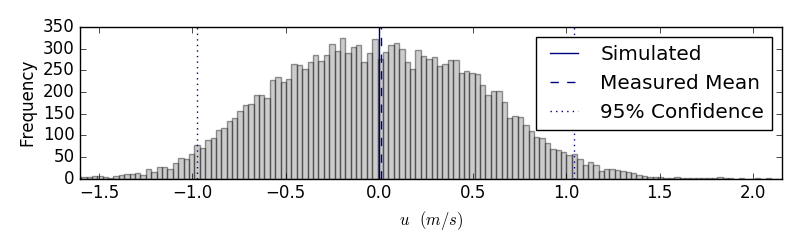
\includegraphics[width=6in]{figs/Ely_May28th02003/uncertainty_Ely_May28th02003_U}
\caption{Histogram of $U$ measurements at station 2. Simulated conditions $(u,v,w)=(0.0, 0.0, 9.0)$, $dt=25 \mu s$, $\beta_U=\pm 0.0089$, $P_U=\pm 0.5362$, $U_U=\pm 1.0723$}
\label{fig:uncertainty_Ely_May28th02003_U}
\end{figure}


\begin{figure}[H]
\centering
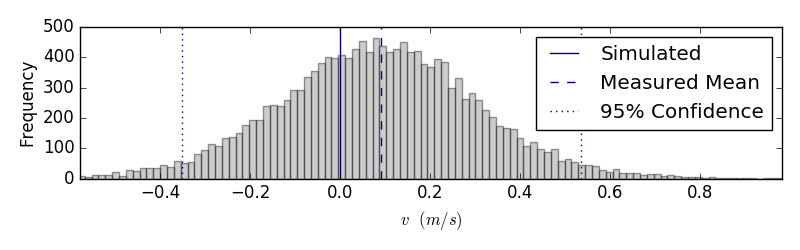
\includegraphics[width=6in]{figs/Ely_May28th02003/uncertainty_Ely_May28th02003_V}
\caption{Histogram of $V$ measurements at station 2. Simulated conditions $(u,v,w)=(0.0, 0.0, 9.0)$, $dt=25 \mu s$, $\beta_V=\pm 0.0908$, $P_V=\pm 0.2226$, $U_V=\pm 0.4543$}
\label{fig:uncertainty_Ely_May28th02003_V}
\end{figure}


\begin{figure}[H]
\centering
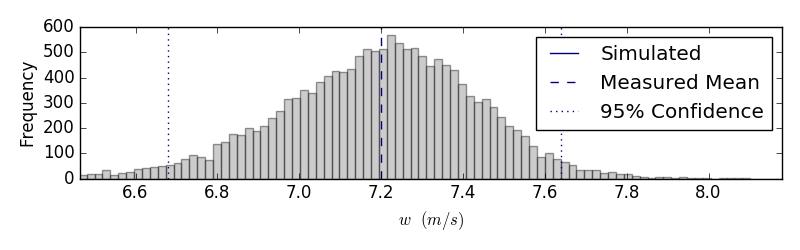
\includegraphics[width=6in]{figs/Ely_May28th02003/uncertainty_Ely_May28th02003_W}
\caption{Histogram of $W$ measurements at station 2. Simulated conditions $(u,v,w)=(0.0, 0.0, 9.0)$, $dt=25 \mu s$, $\beta_W=\pm -1.8001$, $P_W=\pm 0.2449$, $U_W=\pm 1.8656$}
\label{fig:uncertainty_Ely_May28th02003_W}
\end{figure}


